%! Author = NekoHitDev
%! Date = 2021/7/30
%! Language = English (US)
%! compiler = XeLaTex

% Preamble
\documentclass[12pt,a4paper]{article}
\usepackage[T1]{fontenc}

% Packages
\usepackage{amsmath}
\usepackage{url}
\usepackage{graphicx}
\usepackage[slantfont, boldfont]{xeCJK}

% set CJK font
\setCJKmainfont{SimSun}

% include header file
\newcommand{\editversion}{v0.0.1-RC1}

\newcommand{\gentitlepage}[1]{
    \begin{titlepage}
        \centering
        \vfill
        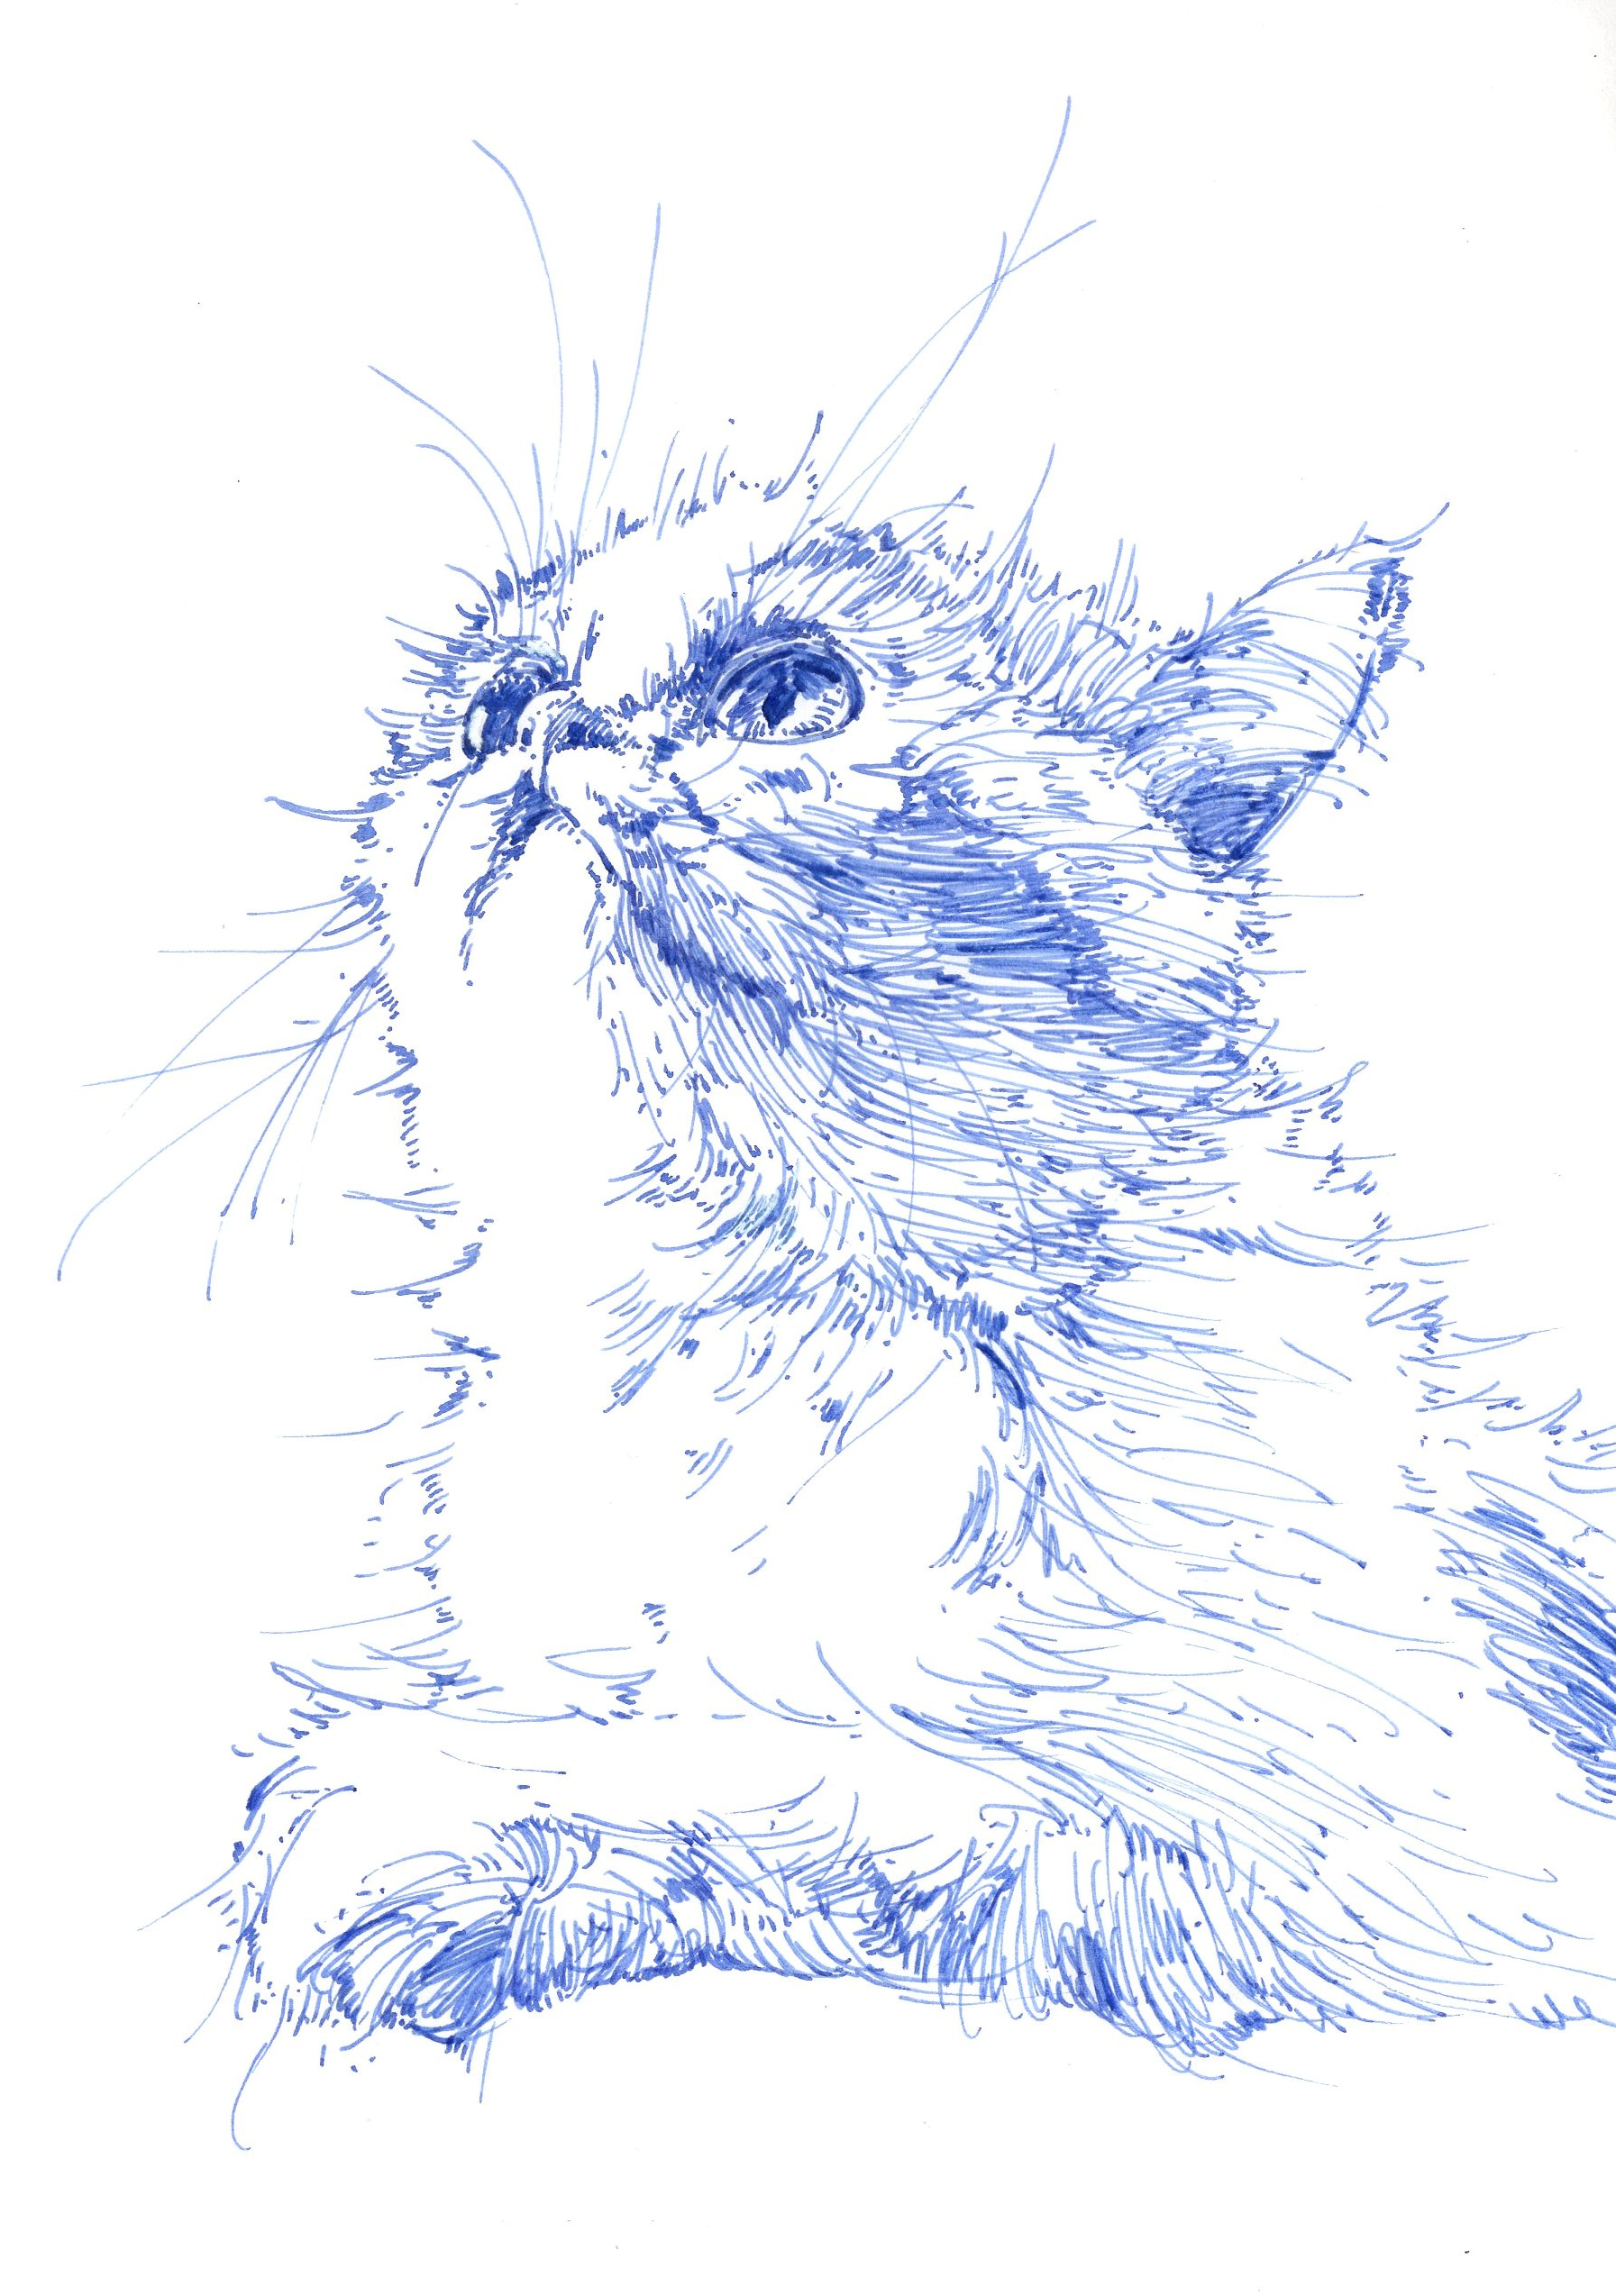
\includegraphics[width=0.8\textwidth]{assets/img196}
        \vfill
        {\Huge
        \textsf{NekoHit Project}\\
        #1\\
        \vskip2cm
        \vfill
        \Large
        \editversion
        }
        \vfill
        \vfill
    \end{titlepage}
}

% TOC stop at subsection
\setcounter{tocdepth}{2}


% Document
\begin{document}
    \gentitlepage{White paper}
    \pagenumbering{Roman}
    \tableofcontents
    \vspace*{\fill}
    \begin{center}
        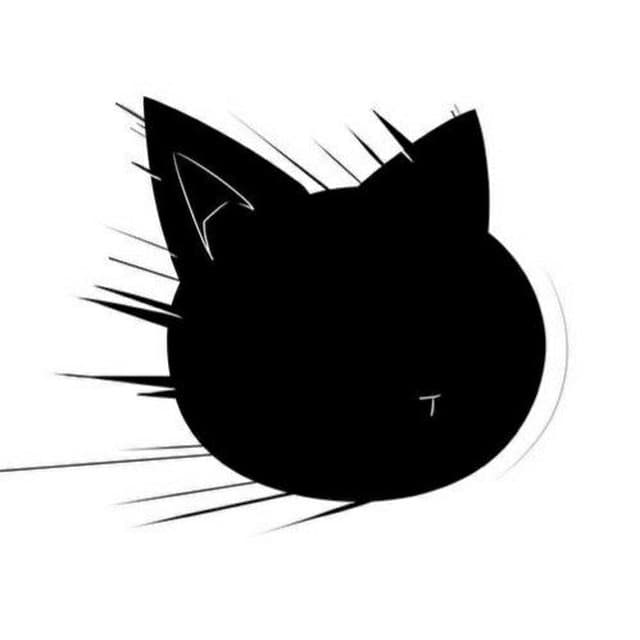
\includegraphics[width=0.67\textwidth]{assets/img197}
    \end{center}
    \clearpage

    \pagenumbering{arabic}


    \section{Vision of the future}\label{sec:goal}

    The vision (goal) of the NekoHit Project is to build a decentralized application
    that gives creators the freedom to spend their time and energy, and allows audiences
    to support creators financially, while incentivizing creators to respond to sponsors.

    We envisioned that as more and more creators and sponsors join,
    the NekoHit community will grow and improve. And we, as the developers
    of the app, will work with the community and respond to the needs and
    feedback from the community users, and strive to create an
    energetic platform for creators.


    \section{Introduction}\label{sec:intro}

    The NekoHit Project built on the work completion agreement
    ("WCA" for short), briefly speaking, it is the blockchain version
    of Patreon. The project aims to incorporate \textit{insurance} into
    traditional sponsor model, to promote the willingness of audiences to
    financially support content creators, and motivate creators to comply
    with their promises and get the project finished on time.

    The subscription model of the NekoHit Project is different from Patreon.
    Instead of paying a monthly subscription fee, we allow audience to sponsor
    a project more specifically. In order to gain the trust of audience, content
    creators need to pledge (stake) some tokens first.
    These tokens need to be transferred to our WCA smart contracts
    before the sponsors can transfer the tokens for sponsorship to
    the creator's projects. The sponsored tokens are also held by our WCA contract.
    When declaring a project, the creator needs to provide information such as
    the rate of the staking (pledging), the detailed milestones of the project and
    the expected completion time.
    If the creator does not complete certain milestones by the expected time,
    WCA contract will automatically calculate the percentage of those milestones
    to the project and deduct it from the pre-pledged tokens.
    After the project is completed, the deducted tokens will be released to each
    sponsor in proportion to the reference sponsorship amount. And the tokens
    sponsored by the sponsor will also be deducted by the corresponding percentage
    and returned to the sponsor's wallet as a refund. So not only does the author
    not receive the sponsorship tokens for his defaulted milestone, but he also loses
    some of his own pledged tokens.

    We use this mechanism as a safety net to protect the rights of our sponsors
    and as an incentive for creators to complete their projects according to the
    expected schedule, so that they do not take too long to complete their projects.
    Such a mechanism will also urge the creators to think through the process of
    creating the project and arrange the timeline appropriately.
    Last but not least, we hope that this will increase the trust of audience in the
    content creators and reduce their concerns about financial sponsorship.


    \section{Industry Status}\label{sec:now}

    There is a growing interest in the creator economy, where audiences are
    not only willing to fund creators, but creators also need various sources
    of income to sustain their work. The market related to the creator economy
    is still relatively raw, and this is certainly an opportunity for us to grow.

    \subsection{Subscription-based traditional model}\label{subsec:tradition_patreon}

    The most typical of the traditional subscription-based model is Patreon.
    It is based on a monthly subscription model, where creators can customize
    their plans with different price, and usually the lower price means less returns.
    Take the famous illustrator WLOP for example, his Patreon is divided into five
    types of plans\cite{wlop_patreon}:
    \begin{itemize}
        \item Knight: \$2 per month, with JPG format comics (3000 pixel wide), and wallpaper created that month (4K resolution)
        \item Black Knight: \$4 per month, with full-size comic, and the wallpaper created that month (8K resolution)
        \item Templar: \$8 per month, with everything in Black Knight, and brushes used by a WOLP in Photoshop, and a PSD source files created that month.
        \item Angel: \$14 per month, with everything in the Templar, and 40\% off in illustrator's store, or the dynamic version of wallpaper, as well as the original video of the painting process (1080P, without the double speed), as well as the basic tutorial for the beginning of the month for drawing beginners, with 40\% off when buying the previous tutorials.
        \item Asura: \$20 per month, with everything in Angel, and free access to one of the source files of any previous works, tutorials or dynamic wallpapers per month.
    \end{itemize}\footnote{
        WLOP's Patreon is charged in term, two 2 term per month,
        and the pricing in the table is a monthly fee.
    }

    As of July 30, 2021, WLOP had a total of 5854 sponsors on Patreon, and have
    maintained an average update frequency of two to three times a month.
    However, WLOP is not the only model at Patreon that can be successful.
    Let's take another look at Sonic Ether's Patreon. Sonic Ether is the author
    of Minecraft's famous shader package "SEUS", and currently he is making the
    ray-tracking version for Mincraft Java edition. There are four plans on his
    Patreon\cite{seus_patreon}:

    \begin{itemize}
        \item Stone: \$1 per month, you can join the Discord server and have Stone rights, and get the latest development progress and screenshots.
        \item Iron: \$5 per month, with everything in Stone, and Iron rights in the server.
        \item Gold: \$10 per month, with everything Iron, and Gold rights in the server.
        \item Diamond: \$25 per month, with everything Gold, and Diamond rights in the server.
    \end{itemize}

    As of July 30, 2021, Sonic Ether has a total of 6923 sponsors on Patreon,
    and maintains update every two to three months. It is worth mentioning that
    on July 22, 2021, Sonic Ether changed the policy to access his least work.
    Previously you have to subscript to at least the Gold Plan to the download
    the shader package, but now is available to everyone and no longer require
    a monthly sponsorship. Sonic Ether currently generates \$56939 per month in revenue.

    In both cases, it was the creator who released the work first and then
    moved to Patreon\footnote{
        Sonic Ether started using Patreon on October 14, 2017,
        while his shader packages were released in 2016.
        WLOP started using Patreon on January 15, 2015,
        but his works are released as early as 2014.
    }. This requires content creators who use Patreon
    must release some respective works first, followed by a stable and
    reasonable updating frequency, before it is possible to obtain the
    sponsorship from his audience.
    For a newcomer, or other outcomes such as hardware, which are not
    easy to deliver through the internet, those creators are more likely
    to use the crowdfunding model.

    \subsection{Crowdfunding-based traditional model}\label{subsec:tradition_kickstarter}

    The traditional crowdfunding-based model, in the case of Kickstarter,
    prefers a one-time sponsorship compared to Patreon's monthly subscription.
    A wide variety of crowdfunding projects can be found on Kickstarter's
    website\cite{kickstarter_homepage}, including art exhibitions, comic illustration,
    design, film, video crafts, games, hardware, music, publishing, and so on.

    According to Kickstarter's own introduction\cite{kickstarter_about},
    the platform is dedicated to transforming creative ideas into reality.
    The initiator (creator) of a crowdfunding project will have full
    control over the works, and it is relatively easy to launch a
    crowdfunding project: no project application paper is required, no
    donors asking for changes to the project, and no investors asking
    for changes to the product at the final moment. In general, Kickstarter
    is more in favor to creators, by giving them as much freedom as
    possible to enable them to turn excellent creative ideas into
    real-world products. Such independence can inspire superior
    products, but when it comes to malicious projects, there's little
    supporters can do when they realize they have been fooled.

    Taking the example of Milk Nanny\cite{kickstarter_milk_nanny},
    the project is advertised as a smart milk brewer.
    To use it, all you need to do is open the mobile app, enter the
    child's birth year, and scan the barcode of the milk powder,
    and it will automatically brew it in less than a minute.
    The project raised 120 thousand dollar, but judging from the
    project's comments, the product did not materialize and the sponsors
    never received a milk brewer or a refund.

    Also the same unfinished project: Cabin project\cite{kickstarter_cabin},
    which is advertised as one of the most convenient ways to charge the iPhone.
    The project received more than 188 thousand dollar, and only a small number of
    sponsors received the product after 8 months of the scheduled time, and
    many of them were not able to use it as advertised. And the rest sponsors
    never received the product, and the project hasn't been updated on
    the Kickstarter since then.

    \subsection{Summary for traditional models}\label{subsec:tradition_summary}

    The traditional crowdfunding model puts all the initiative on the creator,
    once the sponsor pays the sponsored money, the money will go straight
    into the creator's account, after which sponsors will have no control on
    the project, no matter it can be completed or be refunded, or never updated again.
    For monthly subscription, while sponsors can stop subscribing from next month,
    for sponsors who already subscribe to some plan, the only thing they can do is stop
    the subscription if the creator don't do anything or delivered a less-quality work.

    Traditional models are not the whole story. With the blockchain technology
    as well as the cryptocurrency gradually accepted by public, others have tried
    to implement creator economy on the blockchain.

    \subsection{瞬matataki}\label{subsec:blockchain_matataki}

    The 瞬matataki platform is intended to help free creators
    gain more revenue and build a publicly perpetual library of
    digital works. The platform proposes the concept of
    Fan tickets and personal tokens. Fan tickets are built based
    on the Ethereum Rinkeby test network, and each person can issue
    their own Fran tickets. Those Fans tickets can be held and consumed
    by others (for unlocking the issuer's article)\cite{mitataki_fan_ticket}.

    The platform focuses on the freedom of creation. By issuing
    individual tokens on their platform, the audiences can exchange legal tender
    for the creator's tokens and purchase for access to creator's work in the future.
    The platform also stores creators' work on IPFS\cite{ipfs},
    which allows decentralized storage and avoids potential content censorship.

    The flexible currency model gives more possibilities to 瞬matataki platform,
    but we believe that an overly flexible currency model would place an
    unnecessary burden on content creators. And as of now, there is no way to
    interact directly with the Ether Rinkeby test network or IPFS nodes to use
    the platform outside of their own website, which is a centralized application.
    Also, since the platform relies on the Rinkeby test network for no-fee
    transactions, migrating to the main Ethernet network would result in high
    fees per transaction, which would prevent users from using their personal
    tokens for small transactions on the platform. But staying on the test network
    requires the platform to guarantee the value of individual tokens.


    \section{Our solution}\label{sec:solution}

    In the previous section, we cited two traditional application and a platform
    built on blockchain. We summarized the advantages and disadvantages of these
    three models and propose the NekoHit Project. The project consists of two
    key components: the work completion agreement (WCA) and the completion agreement
    tokens (CAT). Our project focuses on the implementation of a sponsorship
    platform that is simple and easy to use, and gives users (both creators
    and sponsors) the power and ability to protect their rights and
    interests. At the same time we want to be as open as possible: we do not
    restrict what platform the creator uses to store the work, nor restrict
    how user invoke our contracts, and in the future we will also do our best
    to implement the free choice of other token, aka no limitation on what token
    they use to pledge and sponsor.

    \subsection{Work Complete Agreement}\label{subsec:wca}

    The Work Completion Agreement (WCA) is the core feature of the
    NekoHit Project. WCA based on the individual projects, and
    gives sponsors more control compared to traditional models,
    in addition to being able to make a refund \footnote{
        Refunds depend on the progress of the project and
        in some cases full refunds are not possible.
    } at any time, it also provides an insurance-like mechanism
    that automatically refunds to sponsor's wallet when the creator fails
    to meet the the schedule, and penalizes the creator.
    The WCA and the specific mechanism are explained below.

    \subsubsection{Overview}

    One complete use process of the WCA is as follows:

    \begin{enumerate}
        \item The creator calls the WCA Contract to declare a project
        \item The creator calls the CAT contract to transfer pledged tokens
        \item Audiences call for CAT contract transfer to sponsor project\label{item:purchase_wca}
        \item The creator calls the WCA contract to update the project (update milestone)\label{item:update_milestone}
        \item The creator or sponsor calls the WCA contract to end the project (accounting tokens)\label{item:finish_project}
    \end{enumerate}

    Step~\ref{item:update_milestone} can be called multiple times
    by the creator to update different milestones. The sponsor can
    make a refund at any time, from the moment he starts his sponsorship
    at step~\ref{item:purchase_wca}, until the end of project before
    step~\ref{item:finish_project}, but the amount of the refund can
    vary from full to partial depending on the project's progress.

    \subsubsection{Declare project}

    Declaring a project refers to bind the given project information
    with the unique identifier and register to WCA contract.
    The project information is the requested as follows:

    \paragraph{Creator's ScriptHash}

    ScriptHash is generated by the Neo N3 wallet address,
    each address corresponding to the unique ScriptHash,
    which can be understood as a contract-oriented address.
    WCA contract needs to track the address to confirm that
    operations such as updates can only be called by the
    project's creator.

    \paragraph{Description of project}

    A brief introduction to the project. It is important to note
    that every byte of data stored on the Neo N3 blockchain consume
    Gas, so please try to be brief and concise, or give a
    link such as the project presentation URL, IPFS CID, etc.

    \paragraph{Stake (pledge) rate}

    Will determine the total amount of the pledge, and the ratio
    of the payout when creator miss a milestone.

    \paragraph{The maximum amount of sponsorship}

    The upper limit of total sponsorship amount. The sponsored tokens
    from all sponsors on this project cannot exceed that value.

    \paragraph{List of milestones}

    The detailed definition of project milestones.
    Each milestone has three fields: title, introduction and
    expected completion time. The expected completion time
    is stored as timestamp, with maximum accuracy of milliseconds.
    Among the many milestones, there is a special milestone
    referred as threshold milestone.

    For all milestones, the expected completion time of the previous
    milestone should always earlier than the latter one.

    \paragraph{Threshold milestone}

    This is specified by the creator. This milestone determines the
    behavior when sponsor request a refund.
    If refund is requested before this milestone is completed, the sponsor can get a
    full refund. If refund is requested after this milestone is completed,
    only the percentage of milestones that creator has not completed
    will be refunded, and the penalty rule is not applicable.

    \paragraph{Update Cool-down interval}

    This value determines the shortest interval between two milestone updates.
    The creator must wait for this time before they can update (complete)
    the next milestone. The introduction of cooling time is to protect the
    sponsors, so they can notice the malicious projects and have time to make
    refunds. Since the minimum update interval varies from project to project,
    the cooling time will be specified by the creator and displayed in a clear
    way when the sponsor sponsors the project, and it is up to the sponsor to
    decide whether to believe the creator for shorter cooling time.

    \paragraph{Should be public}

    This field indicate whether the contract will list your project publicly.
    But do be aware that all the data stored on the Neo N3 blockchain is open and
    transparent, meaning that anyone can read all the project data by directly access
    the storage of the smart contract. So setting this to "no" cannot prevent your
    project from being accessed by unknown entity.

    \paragraph{Unique identifier}

    This field determines how the sponsor finds the project.
    The identifier is also the key for subsequent interaction with the contract,
    to specify a project to operate. The identifier must be unique across the network.
    If the given identifier is duplicated, the contract will throw an exception
    to mark this transaction invalid.

    \subsubsection{Stake (pledge) token}

    Staking token is required after creator declare his project,
    by transferring the specified amount of tokens to the WCA contract,
    before allowing the sponsor to purchase it. If anyone attempt to sponsor or operate
    an unpaid project, the contract will throw an exception and make the transaction invalid,
    so user's assets will be safe.

    The calculation formula of the specified amount is as follows:
    $\text{total stake} = \text{stake rate} \times \text{maximum amount of sponsorship}$

    Assuming A project with the maximum sponsorship amount of 1000 tokens and
    the stake rate is 0.5, then a total of 500 tokens will be required.

    Currently, WCA contract only supports the CAT tokens.

    \subsubsection{Sponsor a project}

    After the creators complete the stake, he or she can advertise their projects
    on other platforms. Sponsors can sponsor the project using the identifier.

    When do the sponsor,you have to transfer tokens to WCA contract with identifier
    as the fourth parameter (aka the data param), so WCA contract can record your
    sponsorship to this specific project. If the identifier does not exist or not
    available for purchase, the contract will throw an exception to make this
    transaction invalid. Your assets will be safe.

    A project is available to sponsor only if:
    the creator has paid the stake and, the first milestone has not been completed nor expired.

    \subsubsection{Updating project}

    The creator may invoke the WCA contract at any time to update the milestone of the project.
    Updating a milestone will prevent new sponsors from sponsoring the project,
    but it won't affect refund requests for existing sponsors.
    When updating the project, only subsequent milestones is allowed to update,
    creator cannot update the milestones that have already passed.

    Example: Milestone \#1 and \#3 is finished, so milestone \#2 cannot be updated
    even if it is not expired.

    A piece of text is required when updating the milestone. Since every byte stored
    on the Neo N3 blockchain consumes GAS, we don't recommend storing your work
    directly in the blockchain. This text can be a URL, or an IPFS CID, or a piece of
    description that guides your sponsors to find your work. If the Sponsor fails to
    find your work through this text, they may assume that you started completing the
    milestone in bad faith and consider a refund. Milestones can not be modified once
    they are updated, so please double-check this text before formally approve the transaction.

    Also: all data stored on the Neo N3 blockchain is open and transparent, which means
    that your text can be read by anyone (including previously refunded sponsors).

    \subsubsection{Refund}

    Sponsors can initiate a refund at any time before the end of the project
    and the refund will be automatically processed by the contract without
    waiting for the consent of the administrator or creator.
    The specific refund rules are as follows:

    If the threshold milestone has not been completed, you can make a
    full refund at any time, and your sponsor record will be deleted
    after the refund. The creator will not be aware of your refund unless
    he review the transaction record of the blockchain.

    If the threshold milestone for the project has already been passed (
    in the meaning of expired or finished by creator),
    you can only get the proportion corresponding to the milestones that
    the creator has not yet completed. Take the following project as an example:
    there are total of 10 milestones, the first number is 1, the last number is 10 and
    the threshold milestone is 3. The milestone 1, 2 and 4 is finished,
    milestone 3 and rest of them have not been completed. Milestone 3 as the
    threshold milestone, even it is not been finished nor expire, since milestone 4
    has been completed, it is considered that milestone 3 has been passed,
    so only partially refund is applicable.

    The refund ratio is: 3 out of 10 is completed by the creator,
    so 30\% of the sponsored token will be sent directly to the creator,
    and the remaining 70\% will be refund to the sponsor's address.
    At the final accounting, milestone 3 will be considered as unfinished,
    thus 10\% of the pledged tokens will be distributed in proportion to
    each sponsor's amount, but this is not applicable when processing the
    refund. Aka no punishment for creator when doing the refund.

    \subsubsection{Ending the project}

    Ending the project will trigger WCA contract to account the property
    and begin to transfer tokens to each related accounts. Take the
    following project as an example: the maximum sponsorship amount
    is 5000 and the stake rate is 0.2, there are 10 milestones
    in total, and the creator completed 7 of them, the creator staked 1000 tokens.

    User A sponsored 500 tokens, user B sponsored 1000 tokens, and user C sponsored 300 tokens.

    When doing the accounting, the stake amount corresponding to user A
    is $500 \times 0.2 = 100$ tokens, so the total amount of user A is
    500 tokens sponsored and 100 tokens staked from creator, a total of 600 tokens.
    The creator didn't finish 3 milestones, so 30\%, aka 180 tokens transferred to user A.
    Similarly, user B will receive a refund of 360 tokens, and user C will receive 108 tokens.

    For the part that returned to the creator, it is calculated as follows:
    the staked part plus the total sponsored amount, i.e.
    $1000 + 500 + 1000 + 300 = 2800$ tokens, subtract those tokens transferred to the Sponsor,
    the remaining $2800 - 180 - 360 - 108 = 2152$ tokens, which will be
    transferred to the creator in one transaction to save Gas.

    \subsection{Completion Agreement Token}\label{subsec:cat}

    Completion Agreement Token (CAT) is the governance token
    issued by the NekoHit Project. The CAT token is also the
    only token accepted by WCA contract for now.

    The CAT tokens supplied with fixed amount of 1,000,000,000
    CAT, with a precision of two decimal places, in line with
    the real world legal tender. The initial issue allocation
    ratio is as follows:

    \begin{itemize}
        \item Community members: 68.64\%
        \item NekoHitDev team: 20.36\%
        \item Investors (if we have any): 9.85\%
        \item Other usage including airdrops: 1.15\%
    \end{itemize}


    \section{Epilogue}\label{sec:end}

    \begin{quotation}
        "NekoHit" was just a random name translats to "cat punch".
        Just as the project was born out of a sudden idea
        from an unknown novel author (Wakayume) while walking.
        After talking with a programmer who had just tried
        blockchain development (Sky Blond) at Misskey,
        The project took a very primitive shape after a simple development.

        Then we went to a hackathon organized by the Neo foundation,
        and the original purpose was just have a try, and on the way we
        met Yannick Koitzsch, a great teammate doing the development along
        with us. At the end it was a great honor that we received the excellent
        award from the Neo Frontier Launchpad.

        I know that we and NekoHit Project are still very young and inexperienced.
        But because we have tried and worked hard, we have been able to grow and
        evolve during the process. I would also like to thank everyone who has
        supported and encouraged us, because of you, we are able to keep going.

        The Excellent award from Neo Frontier Launchpad is just the first step
        we have taken, and I believe we will go further than we ever thought
        possible.

        Please look forward to us.

        \rightline{—— Aozora Wakayume}
    \end{quotation}

    \clearpage

    \bibliography{main}
    \bibliographystyle{IEEEtran}

\end{document}
